%%%%%%%%%%%%%%%%%%%%%%%%%%%%%%%%%%%%%%%%%%%%%%%%%%%
%% LaTeX book template                           %%
%% Author:  Amber Jain (http://amberj.devio.us/) %%
%% License: ISC license                          %%
%%%%%%%%%%%%%%%%%%%%%%%%%%%%%%%%%%%%%%%%%%%%%%%%%%%

\documentclass[a4paper,11pt]{book}
\usepackage[T1]{fontenc}
\usepackage[utf8]{inputenc}
\usepackage{lmodern}
\usepackage{hyperref}
\usepackage{graphicx}
\usepackage[portuguese]{babel}

% coding examples in latex file
\usepackage{listings}
\usepackage{xcolor}

\definecolor{codegreen}{rgb}{0,0.6,0}
\definecolor{codegray}{rgb}{0.5,0.5,0.5}
\definecolor{codepurple}{rgb}{0.58,0,0.82}
\definecolor{backcolour}{rgb}{0.95,0.95,0.92}

\lstdefinestyle{mystyle}{
    backgroundcolor=\color{backcolour},   
    commentstyle=\color{codegreen},
    keywordstyle=\color{magenta},
    numberstyle=\tiny\color{codegray},
    stringstyle=\color{codepurple},
    basicstyle=\ttfamily\footnotesize,
    breakatwhitespace=false,         
    breaklines=true,                 
    captionpos=b,                    
    keepspaces=true,                 
    numbers=left,                    
    numbersep=5pt,                  
    showspaces=false,                
    showstringspaces=false,
    showtabs=false,                  
    tabsize=2
}

\lstset{style=mystyle}


% inserting images
\usepackage{graphicx}

%%%%%%%%%%%%%%%%%%%%%%%%%%%%%%%%%%%%%%%%%%%%%%%%
% Chapter quote at the start of chapter        %
% Source: http://tex.stackexchange.com/a/53380 %
%%%%%%%%%%%%%%%%%%%%%%%%%%%%%%%%%%%%%%%%%%%%%%%%
\makeatletter
\renewcommand{\@chapapp}{}% Not necessary...
\newenvironment{chapquote}[2][2em]
  {\setlength{\@tempdima}{#1}%
   \def\chapquote@author{#2}%
   \parshape 1 \@tempdima \dimexpr\textwidth-2\@tempdima\relax%
   \itshape}
  {\par\normalfont\hfill--\ \chapquote@author\hspace*{\@tempdima}\par\bigskip}
\makeatother


% tirando identação dos paragrafos
\setlength{\parindent}{0ex}

%%%%%%%%%%%%%%%%%%%%%%%%%%%%%%%%%%%%%%%%%%%%%%%%%%%
% First page of book which contains 'stuff' like: %
%  - Book title, subtitle                         %
%  - Book author name                             %
%%%%%%%%%%%%%%%%%%%%%%%%%%%%%%%%%%%%%%%%%%%%%%%%%%%
% Book's title and subtitle
\title{\Huge \textbf{Think Python} \\ 
\Large How to think like a computer scientist \\
\large Second Edition \\
\huge by Allen B. Downey}

% Author
\author{\textsc{Resumo por Bruno de M. Ruas}}


\begin{document}

\frontmatter
\maketitle

\tableofcontents
%\listoffigures
%\listoftables

\mainmatter

%%%%%%%%%%%%%%%%%%%%%%%%%%%%%%%%%%%%%%%%%%%%%%%%%%%
%                 CHAPTER                         %
%%%%%%%%%%%%%%%%%%%%%%%%%%%%%%%%%%%%%%%%%%%%%%%%%%%
\chapter{O Caminho do Programa}

\begin{chapquote}{página 1}
	``The single most important skill for a computer scientistis \textbf{problem solving}. That is the 
	ability to formulate problems, think creatively about solutions, and express a solution clearly and 
	accurately''
\end{chapquote}

\section{O que é um Programa?}
Um \textbf{programa} é uma sequencia de instruções que especifica como fazer um determinado computation. Um \textbf{computation}\footnote{\href{https://en.wikipedia.org/wiki/Computation}{https://en.wikipedia.org/wiki/Computation}} é qualquer tipo de cálculo que inclua 
passos artiméticos (computação matemática) e não artiméticos (computação simbólica) e que segue uma determinada ordem.
\\
\\
Algumas características comuns em qualquer linguagem de programação:
\begin{itemize}
	\item input $\rightarrow$ dados de teclado, arquivo, rede, etc.
	\item output $\rightarrow$ mostrar dados na tela, salvar em um arquivo, enviar na rede, etc.
	\item math $\rightarrow$ operações matemáticas
	\item conditional execution $\rightarrow$ só executar um pedaço do código após certas condições
	\item repetition $\rightarrow$ reexecutar um pedaço do código com alguma variação
\end{itemize}

\section{Executando o Python}
O \textbf{interpretador} do Python é um programa que lê e executa códigos escritos em Python. Existem duas maneiras\footnote{Essa parte eu to adiantando da página 13} de se executar códigos em Python
a primeira é no modo \textbf{interativo} onde podemos enviar as ordens direto pro interpretador e a segunda em em modo \textbf{script} onde
o interpretador analisa o código inteiro antes de começar o processamento.

\section{Operadores Aritméticos}
\begin{lstlisting}[language=Python, caption=Operadores Básicos]
# Soma
40 + 1

# Subtracao
10 - 1

# Multiplicacao
20 * 10

# Divisao
11 / 1

# Exponenciacao
6 ** 2

\end{lstlisting}

\section{Linguagens Formais e Naturais}

As \textbf{linguagens naturais} são as linguagens que as pessoas usam para se comunicar no dia a dia. São criadas e se modificam organicamente com o passar do tempo.
\\
\\
Por outro lado, as \textbf{linguagens formais} são criadas por pessoas e possuem uma aplicação específica. As linguagens de computação são linguagens formais desenvolvidas para expressar computações.
\\
\\
As linguagens formais possuem regras estritas que chamamos de \textbf{regras de sintaxe}.

\subsection{Regras de Sintaxe}

As regras de sintaxe possuem dois sentidos gerais:
\begin{itemize}
	\item tokens $\rightarrow$ são os elementos da linguagem
	\item estrutura $\rightarrow$ é a regra de combinação dos tokens
\end{itemize}

Quando o interpretador lê um código, ele faz um processo chamado \textbf{parsing} que é justamente entender a estrutura de combinação entre os diferentes tokens presentes no script. No caso do Python a identação faz um papel importante na estrutura.

\section{Debugging}

Os erros em um programa são chamados de \textbf{bugs} e o processo de resolução desses erros é chamado de \textbf{debugging}.

\section{Glossário}
\begin{itemize}
	\item problem solving $\rightarrow$ processo de formular um problema, achar uma solução e expressá-la
	\item high-level language $\rightarrow$ lingaugem desenhada para ser fácil para um humano ler e escrever
	\item low-level language $\rightarrow$ lingaugem desenhada para ser fácil para um computador ler. AKA "machine language" ou "assembly language"
	\item portability $\rightarrow$ capacidade de um programa rodar em mais de um tipo de computador
	\item interpreter $\rightarrow$ um programa que lê outro programa e o executa
	\item prompt $\rightarrow$ caracteres no prompt que indicam que ele está pronto para receber input direto do usuário
	\item program $\rightarrow$ um conjunto de instruções que especifica uma computation
	\item print statement $\rightarrow$ uma instrução que diz para o interpretador mostrar caracteres na tela
	\item operator $\rightarrow$ um caracter especial que representa uma computação simples (+, -, *, /, ** ) 
	\item value $\rightarrow$ uma das unidades básica de dados
	\item type $\rightarrow$ a categoria em que um valor pertence
	\item interger $\rightarrow$ numero inteiros
	\item floating-point $\rightarrow$ números fracionados
	\item string $\rightarrow$ sequencia de caracteres
	\item natural language $\rightarrow$ linguagem humana
	\item formal language $\rightarrow$ linguagem com objetivo e regras específicos
	\item token $\rightarrow$ um dos elementos básicos de uma linguagem formal, análogo à palavra na linguagem natural
	\item syntax $\rightarrow$ as regras de estrutura de um programa
	\item parse $\rightarrow$ processo de examinar um programa e analisar sua estrutura
	\item bug $\rightarrow$ um erro no programa
	\item debugg $\rightarrow$ o processo de resolver um erro
\end{itemize}

%%%%%%%%%%%%%%%%%%%%%%%%%%%%%%%%%%%%%%%%%%%%%%%%%%%
%                 CHAPTER                         %
%%%%%%%%%%%%%%%%%%%%%%%%%%%%%%%%%%%%%%%%%%%%%%%%%%%
\chapter{Variáveis, Expressões e Statements}

\begin{chapquote}{página 11}
	``One of the most powerful features of a programming language is the ability to manipulate \textbf{variables}. A variable is a name that refers to a value''
\end{chapquote}

\section{Statements de atribuição}
\begin{lstlisting}[language=Python, caption=Atribuições para diferentes classes]
# string
message = 'acesse www.economiamainstream.com.br'

# interger
n = 12

# floating point
pi = 3.1415
\end{lstlisting}

\section{Nome de Variáveis}
Os nomes das variáveis podem ser o que você quiser. Contudo, existem algumas regras a serem seguidas: 1) Não podem começar com número; 2) Não pode conter caracteres ilegais (@ , \# ,  etc) e 3) Não podem ser uma \textbf{keyword}.

\subsection{Keywords do Python 3}
Essas são as palavras que o interpretador já reservou como tendo significado e que não podem ser atribuídas como nome para nenhuma variável.

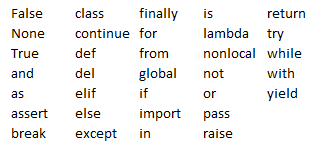
\includegraphics[scale=1]{images/keywords_python.png}

\section{Expressões e Statements}
Uma \textbf{expressão} é uma combinação de valores, variáveis e operadores. Um \textbf{statement} é uma unidade de código que possui algum efeito.

\section{Ordem de Operações}
Python segue a convenção matemática \textbf{PEMDAS}:
\begin{itemize}
	\item \textbf{P}arênteses
	\item \textbf{E}xponenciação
	\item \textbf{M}ultiplicação
	\item \textbf{D}ivisão
	\item \textbf{A}dição
	\item \textbf{S}ubtração
\end{itemize}

\section{Operadores de String}
Quando se trata de strings, Python resignifica os operadores matemáticos para operações $``$ similares $"$ ao contexto original dos números.
\begin{lstlisting}[language=Python, caption=Operadores com strings]

# operador de soma em strings
'economia' + ' ' + 'mainstream'
>>> 'economia mainstream'

# operador de multiplicacao em strings
'economia' * 3
>>> 'economiaeconomiaeconomia'

\end{lstlisting}

\section{Comentários}
Para comentar alguma parte do seu código use o caracter \#. É recomendado que se use comentários apenas para partes não óbvias do código. Se esforce para que o código seja o mais alto-explicativo possível (o nome das varáveis pode ajudar bastante)

\section{Debugging}
Existem 3 tipos de erros que podem acontecer em um programa: 1) Erros de Sintaxe, 2) Erros de Runtime e 3) Erros Semântico.

\begin{itemize}
	\item Erro de Sintaxe $ \rightarrow $ Relacionados à estrutura da linguagem formal e as regras dessa estrutura e dos tokens. Esse tipo de erro não permite a execução do código.
	\item Erro de Runtime $ \rightarrow $ Um erro que não acontece quando o programa inicia mas, em algum momento durante a execução, aparecem posteriormente (geralmente relacionados às exceções não previstas).
	\item Erro de Semântica $ \rightarrow $ O código roda sem erros aparentes, mas o resultado (output) é diferente do esperado. Esse tipo de erro é mais difícil de identificar e de se solucionar. 
\end{itemize}

\section{Glossário}
\begin{itemize}
	\item variable $ \rightarrow $ um nome referente a um valor
	\item assignment $ \rightarrow $ um statement que atribui uma variável a um valor
	\item state diagram $ \rightarrow $ representação gráfica de assignment
	\item keyword $ \rightarrow $ palavras (tokens) reservados pela lingagem para ações previamente definidas
	\item operand $ \rightarrow $ um valor que será usado em uma operação
	\item expression $ \rightarrow $ combinação de variáveis, operadores e valores que representa um único resultado
	\item evaluate $ \rightarrow $ processo de simplificação de uma expressão usando os operadores na ordem correta até chegar em um único resultado
	\item statement $ \rightarrow $ uma parte do código que representa um comando ou uma ação
	\item execute $ \rightarrow $ computar um statement para produzir o resultado por ele ordenado
	\item interactive mode $ \rightarrow $ maneira de interagir com o interpretador do Python escrevendo o input diretamente no prompt
	\item script mode $ \rightarrow $ maneira de interagir com o interpretador do Python através da leitura de um script.py
	\item order of operations $ \rightarrow $ regras de resolução das expressões de acordo com os tokens contidos nos comandos
	\item concatenate $ \rightarrow $ juntar dois ou mais strings
	\item comment $ \rightarrow $ lançamento no script de comentários para facilitar a leitura humana do código. O interpretador não usará essas partes no processamento
	\item syntax error $ \rightarrow $ um erro que torna o processo de parse impossível e, por isso, impede a execução do programa
	\item execption $ \rightarrow $ erro de runtime. Geralmente acontece por uma exceção não prevista no código
	\item semantics $ \rightarrow $ o sentido de um programa
	\item semantic error $ \rightarrow $ um erro onde o programa é executado mas não produz os outputs esperados
\end{itemize}


%%%%%%%%%%%%%%%%%%%%%%%%%%%%%%%%%%%%%%%%%%%%%%%%%%%
%                 CHAPTER                         %
%%%%%%%%%%%%%%%%%%%%%%%%%%%%%%%%%%%%%%%%%%%%%%%%%%%
\chapter{Funções}

\begin{chapquote}{página 21}
	``A \textbf{function} is a named sequence of statements that performs a computation. [...] You specify the name and the sequence of statements. Later, you `call' the function by name.''
\end{chapquote}

\section{Chamadas de Funções}
Uma função possui um \textbf{nome} e, normalmente, recebe \textbf{argumentos}. O resultado obtido após a chamada de uma função com os devidos argumentos é o seu \textbf{valor de retorno}. O Python já possui internamento várias funções que são muito úteis para os desenvolvedores. 

\section{Funções Matemáticas}
Um \textbf{module} é um conjunto de funções e variáveis. Essas funções ficam disponíveis ao interpretador por meio de um \textbf{statement de importação}. O Python possui nativamente um module de operações matemáticas. Para acessar as funções e 

\begin{lstlisting}[language=Python, caption=Carregando o module math]

import math


\end{lstlisting}


















%%%%%%%%%%%%%%%%%%%%%%%%%%%%%%%%%%%%%%%%%%%%%%%%%%%
%                 CHAPTER                         %
%%%%%%%%%%%%%%%%%%%%%%%%%%%%%%%%%%%%%%%%%%%%%%%%%%%
\chapter{Case Study: Interface Design}
\chapter{conditionals and Recursion}
\chapter{Fruitful Funtions}
\chapter{Iteration}
\chapter{Strings}
\chapter{Case Study: Word Play}
\chapter{Lists}
\chapter{Dictionaries}
\chapter{Tuples}
\chapter{Case Study: Data Structure Selection}
\chapter{Files}
\chapter{Classes and Objects}
\chapter{Classes and Functions}
\chapter{Classes and Methods}
\chapter{Inheritance}
\chapter{The Goodies}
\chapter{Debugging}
\chapter{Analysis of Algorithms}


\end{document}